% ============================================================
%  Agentic Mesh -- System Architecture Diagram
%  Compile:  pdflatex architecture_diagram.tex
%  Or paste the tikzpicture block into Overleaf.
% ============================================================
\documentclass[tikz,border=20pt]{standalone}
\usepackage{tikz}
\usetikzlibrary{
    shapes.geometric,
    arrows.meta,
    positioning,
    calc,
    fit,
    backgrounds
}

%--- colour palette -------------------------------------------
\definecolor{OpBlue}{RGB}{219,234,254}
\definecolor{OpBorder}{RGB}{37,99,235}
\definecolor{PlBlue}{RGB}{224,242,254}
\definecolor{PlBorder}{RGB}{2,132,199}
\definecolor{PlHead}{RGB}{3,105,161}
\definecolor{ExGreen}{RGB}{209,250,229}
\definecolor{ExBorder}{RGB}{13,148,136}
\definecolor{ExHead}{RGB}{15,118,110}
\definecolor{MeshPurple}{RGB}{237,233,254}
\definecolor{MeshBorder}{RGB}{109,40,217}
\definecolor{StoreAmber}{RGB}{254,243,199}
\definecolor{StoreBorder}{RGB}{180,83,9}
\definecolor{SubBg}{RGB}{255,255,255}
\definecolor{LabelBg}{RGB}{254,249,195}
%--------------------------------------------------------------

\begin{document}
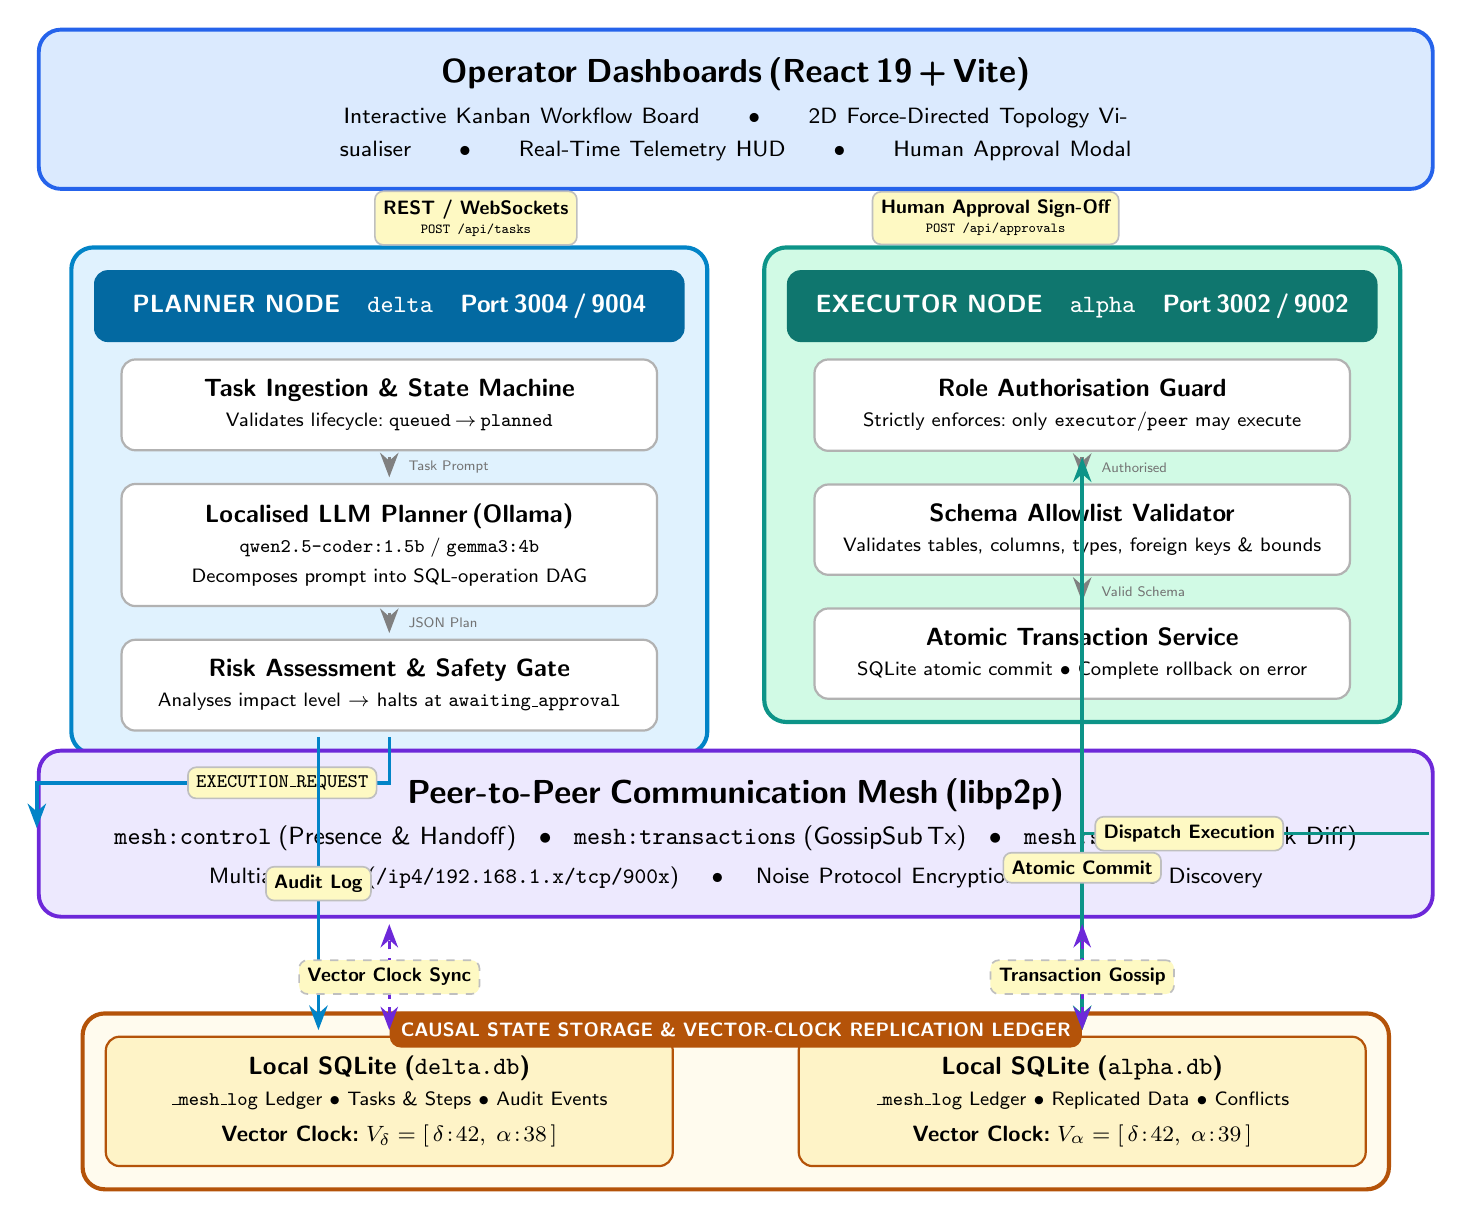
\begin{tikzpicture}[
    font=\sffamily,
    >=Stealth,
    % node styles
    bigbox/.style   = {draw=#1, line width=1.5pt,
                       rounded corners=8pt, inner sep=8pt},
    hdr/.style      = {fill=#1, text=white,
                       font=\bfseries\small\sffamily,
                       align=center, inner sep=6pt,
                       minimum width=7.5cm,
                       minimum height=26pt,
                       rounded corners=5pt},
    sub/.style      = {draw=black!30, fill=SubBg,
                       rounded corners=5pt, line width=0.8pt,
                       align=center, inner sep=7pt,
                       font=\small\sffamily,
                       minimum width=6.8cm},
    % arrow styles
    arr/.style      = {->, line width=1.3pt, draw=#1,
                       shorten >=2pt, shorten <=2pt},
    darr/.style     = {<->, line width=1.2pt, draw=#1,
                       dashed,
                       shorten >=2pt, shorten <=2pt},
    lbl/.style      = {font=\scriptsize\bfseries\sffamily,
                       fill=LabelBg, draw=black!25,
                       line width=0.6pt,
                       inner sep=3pt, rounded corners=3pt},
    slbl/.style     = {font=\tiny\sffamily, text=black!55}
]

% ==============================================================
% 1. OPERATOR DASHBOARD  (top bar)
% ==============================================================
\node[draw=OpBorder, fill=OpBlue,
      rounded corners=8pt, line width=1.4pt,
      align=center, inner sep=10pt,
      text width=17cm, minimum height=1.2cm
] (ui) at (0,0) {%
  \textbf{\large Operator Dashboards\,(React\,19\,+\,Vite)}\\[3pt]
  \footnotesize
  Interactive Kanban Workflow Board
  $\;\bullet\;$ 2D Force-Directed Topology Visualiser
  $\;\bullet\;$ Real-Time Telemetry HUD
  $\;\bullet\;$ Human Approval Modal%
};

% ==============================================================
% 2. PLANNER NODE  delta  (left column)
% ==============================================================
\node[hdr=PlHead] (pl_head) at (-4.4,-2.5)
  {PLANNER NODE\quad\texttt{delta}\quad Port\,3004\,/\,9004};

\node[sub, below=0.2cm of pl_head] (pl_q)
  {\textbf{Task Ingestion \& State Machine}\\
   \scriptsize Validates lifecycle:\;\texttt{queued}$\,\rightarrow\,$\texttt{planned}};

\node[sub, below=0.4cm of pl_q] (pl_llm)
  {\textbf{Localised LLM Planner\,(Ollama)}\\
   \scriptsize\texttt{qwen2.5-coder:1.5b}\;/\;\texttt{gemma3:4b}\\
   \scriptsize Decomposes prompt into SQL-operation DAG};

\node[sub, below=0.4cm of pl_llm] (pl_risk)
  {\textbf{Risk Assessment \& Safety Gate}\\
   \scriptsize Analyses impact level
   $\rightarrow$ halts at \texttt{awaiting\_approval}};

\draw[arr=black!50] (pl_q.south) -- (pl_llm.north)
  node[midway, right=3pt, slbl]{Task Prompt};
\draw[arr=black!50] (pl_llm.south) -- (pl_risk.north)
  node[midway, right=3pt, slbl]{JSON Plan};

\begin{scope}[on background layer]
  \node[bigbox=PlBorder, fill=PlBlue,
        fit=(pl_head)(pl_q)(pl_llm)(pl_risk)
  ] (pbox) {};
\end{scope}

% ==============================================================
% 3. EXECUTOR NODE  alpha  (right column)
% ==============================================================
\node[hdr=ExHead] (ex_head) at (4.4,-2.5)
  {EXECUTOR NODE\quad\texttt{alpha}\quad Port\,3002\,/\,9002};

\node[sub, below=0.2cm of ex_head] (ex_auth)
  {\textbf{Role Authorisation Guard}\\
   \scriptsize Strictly enforces:\;only \texttt{executor}/\texttt{peer} may execute};

\node[sub, below=0.4cm of ex_auth] (ex_val)
  {\textbf{Schema Allowlist Validator}\\
   \scriptsize Validates tables, columns, types, foreign keys \& bounds};

\node[sub, below=0.4cm of ex_val] (ex_atom)
  {\textbf{Atomic Transaction Service}\\
   \scriptsize SQLite atomic commit $\bullet$ Complete rollback on error};

\draw[arr=black!50] (ex_auth.south) -- (ex_val.north)
  node[midway, right=3pt, slbl]{Authorised};
\draw[arr=black!50] (ex_val.south) -- (ex_atom.north)
  node[midway, right=3pt, slbl]{Valid Schema};

\begin{scope}[on background layer]
  \node[bigbox=ExBorder, fill=ExGreen,
        fit=(ex_head)(ex_auth)(ex_val)(ex_atom)
  ] (ebox) {};
\end{scope}

% ==============================================================
% 4. LIBP2P MESH FABRIC  (explicit y = -9.2)
% ==============================================================
\node[draw=MeshBorder, fill=MeshPurple,
      rounded corners=8pt, line width=1.4pt,
      align=center, inner sep=10pt,
      text width=17cm, minimum height=2cm
] (mesh) at (0,-9.2) {%
  \textbf{\large Peer-to-Peer Communication Mesh\,(libp2p)}\\[4pt]
  \small
  \textbf{\texttt{mesh:control}}\;(Presence \& Handoff)
  $\;\bullet\;$
  \textbf{\texttt{mesh:transactions}}\;(GossipSub\,Tx)
  $\;\bullet\;$
  \textbf{\texttt{mesh:sync}}\;(Vector-Clock Diff)\\[2pt]
  \footnotesize
  Multiaddr TCP\;(\texttt{/ip4/192.168.1.x/tcp/900x})
  $\;\bullet\;$ Noise Protocol Encryption
  $\;\bullet\;$ mDNS Discovery%
};

% ==============================================================
% 5. STORAGE LAYER  (explicit y = -12.4)
% ==============================================================
\node[sub, fill=StoreAmber, draw=StoreBorder,
      minimum width=7.2cm
] (db_delta) at (-4.4,-12.6) {%
  \textbf{Local SQLite\;(\texttt{delta.db})}\\
  \scriptsize\texttt{\_mesh\_log} Ledger
  $\bullet$ Tasks \& Steps $\bullet$ Audit Events\\[2pt]
  \footnotesize\bfseries
  Vector Clock:\;$V_{\delta}=[\,\delta\!:\!42,\;\alpha\!:\!38\,]$%
};

\node[sub, fill=StoreAmber, draw=StoreBorder,
      minimum width=7.2cm
] (db_alpha) at (4.4,-12.6) {%
  \textbf{Local SQLite\;(\texttt{alpha.db})}\\
  \scriptsize\texttt{\_mesh\_log} Ledger
  $\bullet$ Replicated Data $\bullet$ Conflicts\\[2pt]
  \footnotesize\bfseries
  Vector Clock:\;$V_{\alpha}=[\,\delta\!:\!42,\;\alpha\!:\!39\,]$%
};

\begin{scope}[on background layer]
  \node[bigbox=StoreBorder, fill=StoreAmber!30,
        fit=(db_delta)(db_alpha)
  ] (sbox) {};
\end{scope}

\node[fill=StoreBorder, text=white,
      font=\bfseries\scriptsize\sffamily,
      inner sep=4pt, rounded corners=4pt,
      anchor=north
] at (sbox.north)
  {CAUSAL STATE STORAGE \& VECTOR-CLOCK REPLICATION LEDGER};

% ==============================================================
% 6. CONNECTORS
% ==============================================================

%--- UI -> Planner (REST / WebSockets)
\draw[arr=PlBorder]
  ([xshift=-3.3cm]ui.south)
  -- node[midway, lbl, align=center]
       {REST / WebSockets\\[-1pt]\tiny\texttt{POST /api/tasks}}
  ([xshift=-3.3cm]ui.south |- pbox.north);

%--- UI -> Executor (Human Approval)
\draw[arr=ExBorder]
  ([xshift=3.3cm]ui.south)
  -- node[midway, lbl, align=center]
       {Human Approval Sign-Off\\[-1pt]\tiny\texttt{POST /api/approvals}}
  ([xshift=3.3cm]ui.south |- ebox.north);

%--- Planner -> Mesh (EXECUTION_REQUEST)
%    Route: straight down then hard-left into mesh.west
\draw[arr=PlBorder]
  (pl_risk.south) -- ++(0,-0.65)
  -| node[near start, lbl, xshift=25pt]{\texttt{EXECUTION\_REQUEST}}
  (mesh.west);

%--- Mesh -> Executor (Dispatch Execution)
\draw[arr=ExBorder]
  (mesh.east) -|
  node[near start, lbl, xshift=-25pt]{Dispatch Execution}
  (ex_auth.south);

%--- Executor -> alpha.db (Atomic Commit)
\draw[arr=ExBorder]
  (ex_atom.south)
  -- node[midway, lbl]{Atomic Commit}
  (db_alpha.north);

%--- Planner -> delta.db (Audit Log)
%    Note: pl_risk also connects to mesh, so we offset x slightly
\coordinate (pl_audit_top) at ([xshift=-0.9cm]pl_risk.south);
\coordinate (pl_audit_bot) at ([xshift=-0.9cm]pl_risk.south |- db_delta.north);
\draw[arr=PlBorder] (pl_audit_top)
  -- node[midway, lbl]{Audit Log}
  (pl_audit_bot);

%--- delta.db <-> Mesh (Vector Clock Sync)
\draw[darr=MeshBorder]
  (db_delta.north)
  -- node[midway, lbl]{Vector Clock Sync}
  (db_delta.north |- mesh.south);

%--- alpha.db <-> Mesh (Transaction Gossip)
\draw[darr=MeshBorder]
  (db_alpha.north)
  -- node[midway, lbl]{Transaction Gossip}
  (db_alpha.north |- mesh.south);

\end{tikzpicture}
\end{document}
